\section{Konzept}\label{sec:konzept}

\subsection{Systemarchitektur}\label{subsec:systemarchitektur}
\subsubsection*{Abgrenzung}

Dieses Kapitel gibt einen Übersicht über die Systemarchitektur als ganzes. Die Architektur beschränkt sich dabei auf die
Anforderungen die innerhalb des Projektrahmens umgesetzt wurden. Komponenten für Teile die Out Of Scope gefallen sind,
werden hier nicht behandelt.

\subsubsection*{Übersicht}

Das cloudbasierte Praxisrufsystem wird in vier Komponenten unterteilt.
Im Zentrum steht eine cloudbasierte Applikation (Cloud Service) welche es ermöglicht Konfigurationen persistent zu verwalten und das Versenden von Benachrichtigungen anhand dieser Konfigurationen koordiniert.
Der Cloud Service benutzt einen externen Messaging Service zum Versenden von Benachrichtigungen. Dabei ist der Messaging Service lediglich für die Zustellung von Benachrichtigungen verantwortlich.
Zur Verwaltung der Konfigurationen wird ein Web Frontend (Admin UI) erstellt. Dieses bietet einem Administrator die Möglichkeit Konfigurationen aus dem Cloud Service zu lesen, erstellen, bearbeiten und löschen.
Die Konfigurationen die über Admin UI und Cloud Service erstellt wurden, werden schliesslich von einem Mobile Client. Mit dem Mobile Client kann der Benutzer Benachrichtigungen an andere Mobile Clients senden.
Welche Benachrichtigungen ein Mobile Client senden kann und an wen diese Benachrichtungen zugstellt werden, wird anhand der Konfiguration aus dem Cloud Service bestimmt.

\begin{figure}[h]
    \centering
    \begin{minipage}[b]{1.0\textwidth}
        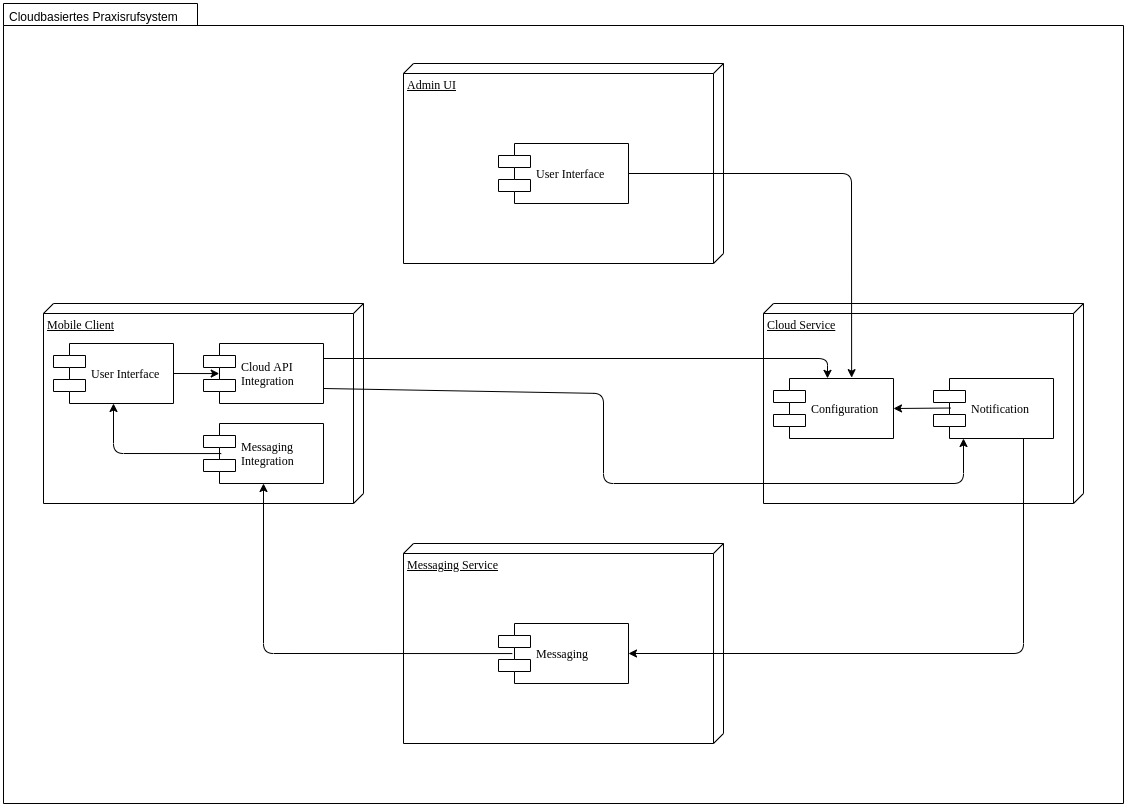
\includegraphics[width=\textwidth]{graphics/Component_System}
        \caption{System}
    \end{minipage}
\end{figure}

\clearpage

Die Anforderungen U12 setzt voraus, dass die Kommunikation im Praxisrufsystem
zwischen mehreren Geräten erfolgen kann.

Die Anforderungen U06, U07 und U13 setzten voraus, dass die es eine zentrale Stelle gibt
die Konfigurationen zur Verfügung stellt und das Versenden von Notifikationen koordiniert.


\subsubsection*{Mobile Client}

\begin{itemize}
    \item Der Mobile Client implementiert die Anbindung an den Messaging Service.
    \item Als Reaktion auf eine Notification wird eine Rückmeldung im UI angezeigt.
    \item Als Reaktion auf eine Notification wird eine OS Push Notifikation gesendet.
    Das UI bietet einen Button der eine Anfrage an die REST Schnittstelle im Cloud Service sendet.
\end{itemize}


\subsubsection*{Cloud Service}

\begin{itemize}
    \item Responsibilities (Notification and Configuration)
    \item Microservice Granularity
\end{itemize}


\subsubsection*{Messaging Service}

\begin{itemize}
    \item Dies wird ein externer Service den wir in die Applikationen einbinden. Standard hierfür ist Firebase Notifications.
    \item Der Messaging Service nimmt Notifikationen vom Cloud Service entgegen und gibt diese an den Mobile Client wieder.
    \item Dafür müssen auf beiden Seiten Komponenten eingebaut werden, die mit dem Messaging Service kommunizieren.
\end{itemize}

\clearpage


\subsection{Mobile Client}\label{subsec:mobile-client}

\subsubsection{Framework Grundlagen}
NativeScript bietet eine Abstraktion zu den nativen Plattformen Android und IOS.
Die jeweilige NativeScript Runtime erlaubt es in Javascript (oder einem entsprechenden Application Framework) Code zu schreiben,
welcher direkt für die entsprechende native Umgebung kompiliert wird~\cite{ns-core-overview}.
\begin{figure}[h]
    \centering
    \label{fig:howNSWorks}
    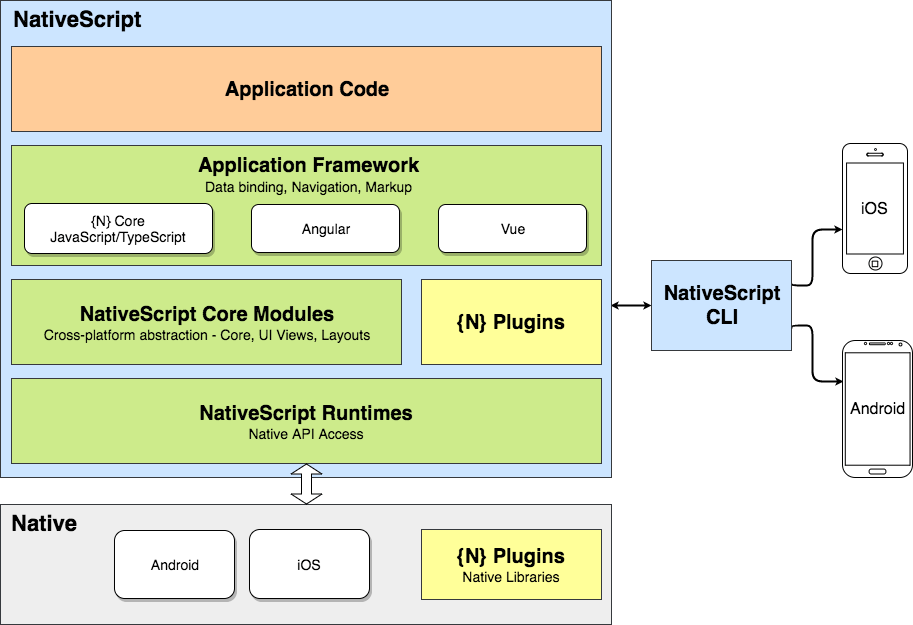
\includegraphics[width=0.7\textwidth]{graphics/ns-common}\caption[NativeScript-Overview]{NativeScript-Overview}\textcopyright OpenJS Foundation
\end{figure}


Die Runtime agiert als Proxy zwischen Javascript und dem jeweiligen Ökosystem.
Im Falle von IOS bedeutet dies u.A. das für alle Objective-C types ein JavaScript Prototype angeboten wird.
Dies ermöglicht es direkt mit nativen Objekten zu interagieren.
Im Umkehrschluss findet eine Typenkonversion via Marshalling Service statt\cite{ns-ios-runtime}.

\subsubsection{Anwendung}
Wir verwenden NativeScript Core als Framework des Mobile-Clients.
In Kapitel~\emph{\nameref{subsec:mobile-client-eval}} gehen wir auf die weiteren verfügbaren Frameworks ein und erläutern, weshalb wir uns gegen sie entschieden haben.

Die Client-Applikation ist in Module unterteilt.
Ein Modul wird aus folgenden Komponenten definiert:
\begin{itemize}
    \item UI-Markup: Statische Darstellung in XML
    \item Backend: Verhalten und Dynamisierung in Javascript
    \item Styling: Layout und Styles in CSS
\end{itemize}

Ein minimales Modul kann alleine aus einer XML-Datei bestehen.
Die optionalen Javascript und CSS Dateien müssen denselben Namen haben wie die XML Datei, um vom Framework korrekt verknüpft zu werden.
Dateien mit anderen Namen werden grundsätzlich vom Framework ignoriert.
Natürlich steht es Frei dennoch solche Dateien anzulegen und deren Funktionen zu verwenden z.~B. als~\emph{\nameref{subsubsec:services}} oder als~\emph{\nameref{subsubsec:code-behind-komponenten}}.

Zur Veranschaulichung der möglichen Interaktionen gehen wir auf die relevanten Aspekte des Home-Screen Modules ein.

\subsubsection*{Page Module}

\dirtree{%
.1 app.
.2 home.
.3 home-page.xml.
.3 home-page.css.
.3 home-page.js.
.3 home-model.js.
}

\emph{\nameref{lst:home-page.xml}} deklariert die umgebenden Komponenten.
Diese Komponenten stellen je nach Typ diverse Properties und Events zur Verfügung.
Properties können entweder statisch befüllt oder aus dem Binding-Context geladen werden.
Den Events können Callback-Functions zugewiesen werden.
Es stehen alle Funktionen zur Verfügung, welche im Backendscript~\emph{\nameref{lst:home-page.js}} exportiert werden.

\lstinputlisting[caption=home-page.xml,language=XML,label={lst:home-page.xml}]{listings/home-page.xml}

Der Binding-Context ist ein JavaScript Objekt welches exklusiv im Page-Context zur Verfügung steht.
Es ist allgemein Best-Practice dieses Objekt in einem eigenen Model zu verwalten.
Das eigentliche Binding wird vom Backendscript~\emph{\nameref{lst:home-page.js}} (Zeilen 8--11) während des ersten Ladens der Seite durchgeführt.

\lstinputlisting[caption=home-model.js,language=JavaScript,label={lst:home-model.js}]{listings/home-model.js}

Das Backendscript ist für das dynamische Verhalten der Seite verantwortlich.
Hier können die Interaktionen der Benutzer beliebig verarbeitet und der Binding-Context bei Bedarf verwaltet werden.

\lstinputlisting[caption=home-page.js,language=JavaScript,label={lst:home-page.js}]{listings/home-page.js}

\subsubsection*{Code-Behind Komponenten}\label{subsubsec:code-behind-komponenten}
Code-Behind Komponenten bieten die Möglichkeit zur Laufzeit dynamisch Grafikelemente dem UI hinzuzufügen.
Komponenten die das Framework bereits zur Verfügung stellt können direkt mit \texttt{new \textless Component\textgreater()} instanziiert werden.
Bei Bedarf können diese Komponenten auch erweitert und mit zusätzlicher Funktionalität ausgestattet werden.

Da der Home-Screen dynamisch in Abhängigkeit der Client-Configuration erstellt werden muss, werden eigene \texttt{MessageTrigger} Komponenten verwendet.
\subsubsection*{Services}\label{subsubsec:services}
In Services werden diejenigen Funktionen ausgelagert, welche nicht direkt im Zusammenhang mit der grafischen Representation stehen.
So z.~B. die REST-Calls zur API.

\clearpage

\subsubsection{Architektur}



\subsubsection{User Interface}
\begin{figure}[h]
    \centering
    \begin{minipage}[b]{0.4\textwidth}
        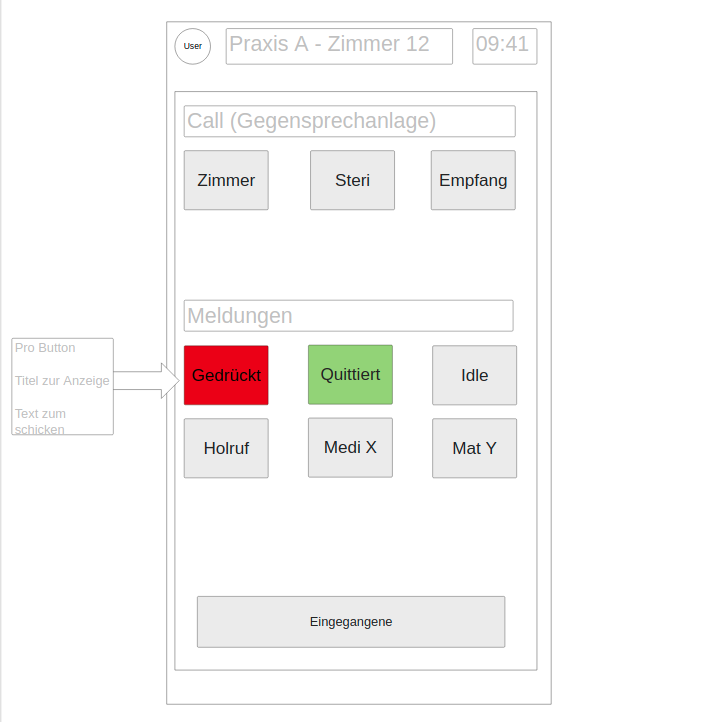
\includegraphics[width=\textwidth]{graphics/homescreen-mockup}
        \caption{HomeScreen Mockup}
    \end{minipage}
    \hfill
    \begin{minipage}[b]{0.4\textwidth}
        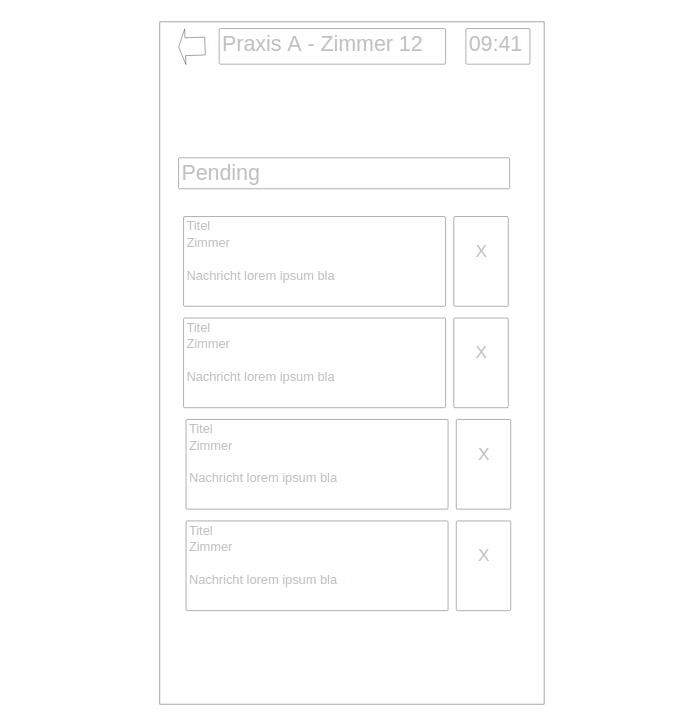
\includegraphics[width=\textwidth]{graphics/mockup-received}
        \caption{Inbox Mockup}
    \end{minipage}\label{fig:MobileClient-Mocks}
\end{figure}


\clearpage


\subsection{Cloud Service}\label{subsec:cloud-service}

\subsubsection{Architektur}

Es gibt deren Domänen 2. Configuration und Notification.

So quasi als ob man 2 Microservices haben kann. Aber wär halt doof das für den stand jetzt schon so zu trennen, deshalb vorerst mal erst ein einzelnes.

\clearpage

\subsubsection{Domänenmodell}


Für die beiden Domänen gibt es natürlich auch so n paar Diagramme. Die gibts jetzt hier:


\subsubsection*{Domäne Configuration}

\begin{figure}[h]
    \centering
    \begin{minipage}[b]{1.0\textwidth}
        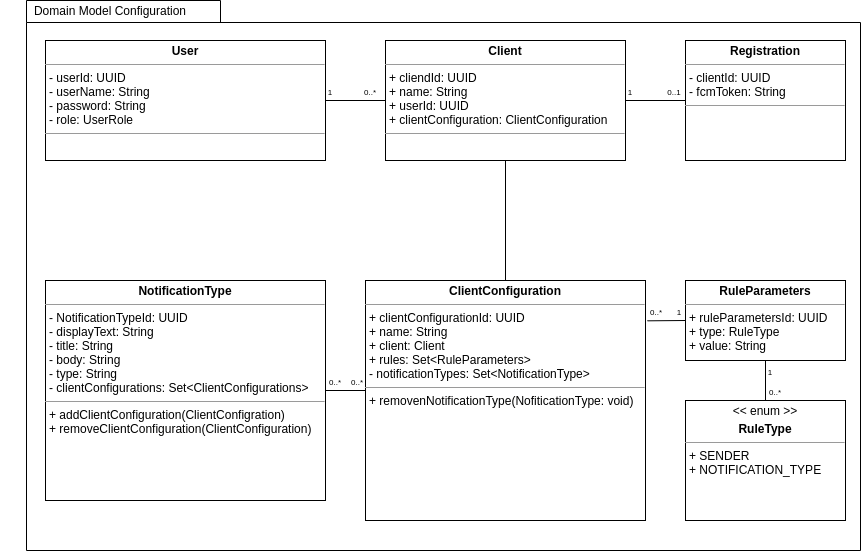
\includegraphics[width=\textwidth]{graphics/Class_Configuration_Domain}
        \caption{Domänenmodell Configuration}
    \end{minipage}
\end{figure}

\clearpage
\subsubsection*{Domäne Notification}

\begin{figure}[h]
    \centering
    \begin{minipage}[b]{1.0\textwidth}
        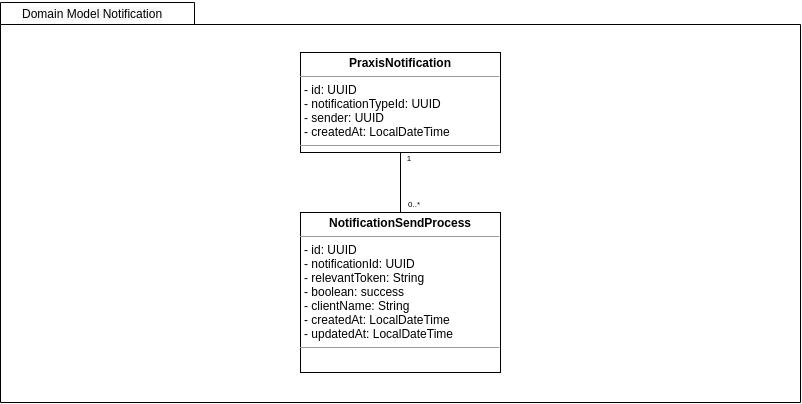
\includegraphics[width=\textwidth]{graphics/Class_Notification_Domain}
        \caption{Domänenmodell Notification}
    \end{minipage}
\end{figure}

\clearpage
\subsubsection*{Rules Engine}

Strategy Pattern mit Spring is noch nice.

\begin{figure}[h]
    \centering
    \begin{minipage}[b]{1.0\textwidth}
        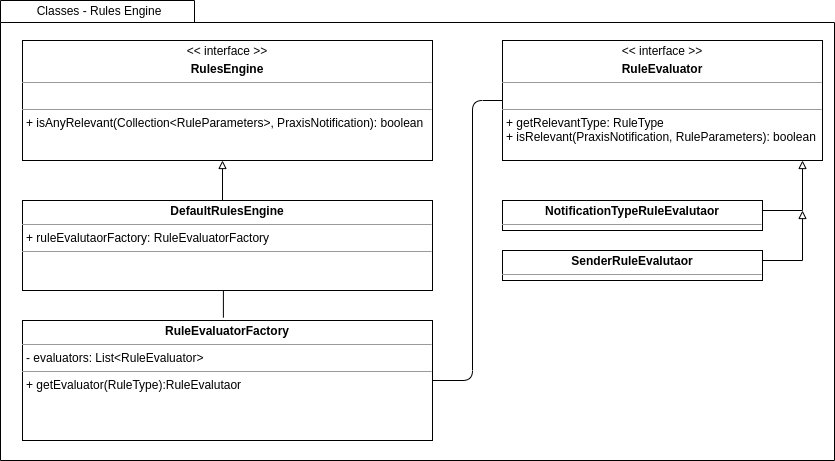
\includegraphics[width=\textwidth]{graphics/Class_Configuration_RulesEngine}
        \caption{Klassendiagramm Rules Engine}
    \end{minipage}
\end{figure}



\clearpage
\subsubsection{API}

S gibt da n paar controller und die brauchen ein paar services.

\clearpage
\subsubsection{Laufzeitmodell}

\clearpage


\subsection{Admin UI}\label{subsec:admin-ui}

\clearpage

\subsection{Proof Of Concept}\label{subsec:poc}

Um sicherzustellen, dass die Anforderungen an das System mit den gewählten Technologien umgesetzt werden können, wird zunächst ein Proof Of Concept implementiert.
Dieser Proof Of Concept hat einen deutlich kleineren Funktionsumfang als das Endprodukt.
Im Wesentlichen muss der Proof Of Concept beweisen, dass es möglich ist mit den gewählten Technologien Benachrichtigungen zu Versenden und zu empfangen.

\subsubsection{Funktionale Anforderungen}

Um dies zu ermöglichen werden die folgenden Features in eingeschränktem Umfang umgesetzt.

\textbf{F01 - Benachrichtigungen Versenden}

Mit dem Proof Of Concept muss es möglich sein, Benachrichtigungen von einem Client zu versenden.
Dementsprechend wird das Szenario "Benachrichtigung versenden" mit den folgenden Einschränkungen umgesetzt:

\begin{itemize}
    \item Es erfolgt kein Login und keine Authentifizierung.
    \item Es gibt nur einen vordefinierten Button.
    \item Es wird immer dieselbe vordefinierte Benachrichtigung versendet.
    \item Es werden keine Empfänger konfiguriert, die Benachrichtigung wird zurück an den Absender versendet.
\end{itemize}


\textbf{F02 - Benachrichtigungen empfangen}

Mit dem Proof Of Concept muss es möglich sein, Benachrichtigungen mit einem Client zu empfangen.
Dementsprechend wird das Szenario "Benachrichtigung empfangen" mit den folgenden Einschränkungen umgesetzt:

\begin{itemize}
    \item Es wird keine Liste von Benachrichtigungen geführt.
    \item Die Benachrichtigung wird in einem einfachen Textfeld im Mobile Client angezeigt.
\end{itemize}


\textbf{F04 - Über Benachrichtigungen Notifizieren}

Mit dem Proof Of Concept muss es möglich sein, über den Einfang von Benachrichtigungen notifiziert zu werden.
Dementsprechend werden die Szenarien "Foreground" und "Background" mit den folgenden Einschränkungen umgesetzt:

\begin{itemize}
    \item Die Notifizierung erfolgt ohne Audio Signal.
\end{itemize}

\clearpage
\subsubsection{Technische Anforderungen}

Damit der Proof Of Concept aussagekräftig ist, müssen die folgenden technischen Anforderungen umgesetzt werden:

\textbf{T01 - IPad Client}

Der für den Proof Of Concept umgesetzte Client muss auf einem IPad funktionieren und alle Anforderungen die an den
Proof Of Concept gestellt werden erfüllen. Kommunikation mit Cloud Service muss funktionieren. Kommunikation mit Messaging Service muss funktionieren.


\textbf{T04 - AWS Platform}

Der Cloud Service muss auf AWS deployed werden. Die Kommunikation zwischen Mobile Client und Cloud Service muss funktionieren.
Die Kommunikation mit Messaging Service muss funktionieren.


\subsubsection{Laufzeitsicht}

Im Wesentlichen muss der Proof Of Concept beweisen, dass es möglich ist mit den gewählten Technologien Benachrichtigungen zu Versenden und zu Empfangen.

Der Benutzer muss den Mobile Client auf dem IPad öffnen können. Aus dem Mobile Client muss der Benutzer über einen Butten eine Benachrichtigung versenden können.
Das Versenden dieser Benachrichtigung erfolgt an den Cloud Service.
Im Rahmen des Proof Of Concept wird eine Benachrichtigung immer an den Sender zurückgesendet. Dabei ist aber wichtig, dass die Benachrichtigung nicht direkt als
Antwort auf die Versenden-Anfrage geschickt wird. Stattdessen muss das Versenden der Benachrichtigung aus dem Cloud Service über den Message Service erfolgen. .

\begin{figure}[h]
    \centering
    \begin{minipage}[b]{1.0\textwidth}
        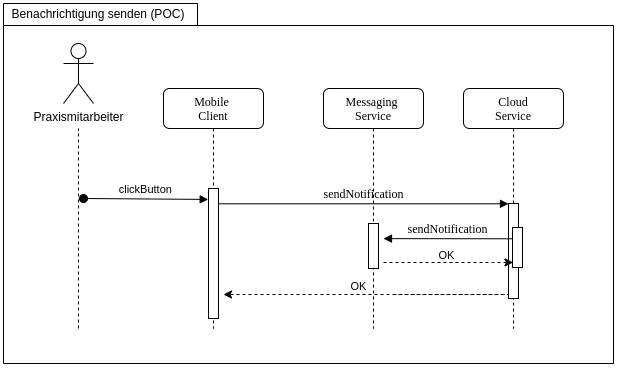
\includegraphics[width=\textwidth]{graphics/Sequence_POC_Send}
        \caption{Proof Of Concept - Benachrichtigung versenden}
    \end{minipage}
\end{figure}

\clearpage


Wurde eine Benachrichtigung über den Message Service an den Mobile Client versendet, muss diese vom Mobile Client empfangen werden.
Als Reaktion auf den Empfang der Benachrichtigung, muss der Inhalt der Benachrichtigung im Mobile Client angezeigt werden. Zudem
muss eine Push Benachrichtigung auf dem Host Gerät erfolgen.

\begin{figure}[h]
    \centering
    \begin{minipage}[b]{1.0\textwidth}
        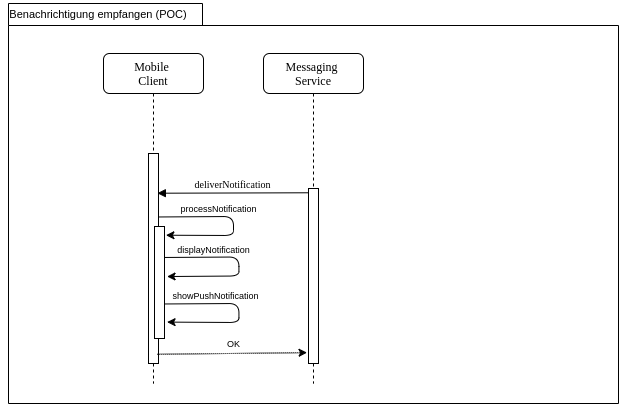
\includegraphics[width=\textwidth]{graphics/Sequence_POC_Receive}
        \caption{Proof Of Concept - Benachrichtigung empfangen}
    \end{minipage}
\end{figure}

\clearpage

